\documentclass[xcolor=table]{beamer}
%\usepackage[utf8]{inputenc}
%\usetheme{Warsaw}
\usetheme{CambridgeUS}
%\usecolortheme{seahorse}

%-------------------------------------------------------------------------------
%          -Packages nécessaires pour écrire en Français et en UTF8-
%-------------------------------------------------------------------------------
\usepackage[utf8]{inputenc}
\usepackage[frenchb]{babel}
\usepackage[T1]{fontenc}
\usepackage{lmodern}
\usepackage{textcomp}

%-------------------------------------------------------------------------------

%-------------------------------------------------------------------------------
%                          -Outils de mise en forme-
%-------------------------------------------------------------------------------
\usepackage{hyperref}
\hypersetup{pdfstartview=XYZ}
\usepackage{enumerate}
\usepackage{graphicx}
%\usepackage{multicol}
%\usepackage{tabularx}

%\usepackage{anysize} %%pour pouvoir mettre les marges qu'on veut
%\marginsize{2.5cm}{2.5cm}{2.5cm}{2.5cm}

\usepackage{indentfirst} %%pour que les premier paragraphes soient aussi indentés
\usepackage{verbatim}
%\usepackage[table]{xcolor}  
%\usepackage{multirow}
\usepackage{ulem}
%-------------------------------------------------------------------------------


%-------------------------------------------------------------------------------
%                  -Nécessaires pour écrire des mathématiques-
%-------------------------------------------------------------------------------
\usepackage{amsfonts}
\usepackage{amssymb}
\usepackage{amsmath}
\usepackage{amsthm}
\usepackage{tikz}
\usepackage{xlop}
\usepackage[output-decimal-marker={,}]{siunitx}
%-------------------------------------------------------------------------------


%-------------------------------------------------------------------------------
%                    - Mise en forme 
%-------------------------------------------------------------------------------

\newcommand{\bu}[1]{\underline{\textbf{#1}}}


\usepackage{ifthen}


\newcommand{\ifTrue}[2]{\ifthenelse{\equal{#1}{true}}{#2}{$\qquad \qquad$}}

\newcommand{\kword}[1]{\textcolor{red}{\underline{#1}}}


%-------------------------------------------------------------------------------



%-------------------------------------------------------------------------------
%                    - Racourcis d'écriture -
%-------------------------------------------------------------------------------

% Angles orientés (couples de vecteurs)
\newcommand{\aopp}[2]{(\vec{#1}, \vec{#2})} %Les deuc vecteurs sont positifs
\newcommand{\aopn}[2]{(\vec{#1}, -\vec{#2})} %Le second vecteur est négatif
\newcommand{\aonp}[2]{(-\vec{#1}, \vec{#2})} %Le premier vecteur est négatif
\newcommand{\aonn}[2]{(-\vec{#1}, -\vec{#2})} %Les deux vecteurs sont négatifs

%Ensembles mathématiques
\newcommand{\naturels}{\mathbb{N}} %Nombres naturels
\newcommand{\relatifs}{\mathbb{Z}} %Nombres relatifs
\newcommand{\rationnels}{\mathbb{Q}} %Nombres rationnels
\newcommand{\reels}{\mathbb{R}} %Nombres réels
\newcommand{\complexes}{\mathbb{C}} %Nombres complexes


%Intégration des parenthèses aux cosinus
\newcommand{\cosP}[1]{\cos\left(#1\right)}
\newcommand{\sinP}[1]{\sin\left(#1\right)}

%Fractions
\newcommand{\myfrac}[2]{{\LARGE $\frac{#1}{#2}$}}

%Vocabulaire courrant
\newcommand{\cad}{c'est-à-dire}

%Droites
\newcommand{\dte}[1]{droite $(#1)$}
\newcommand{\fig}[1]{figure $#1$}
\newcommand{\sym}{symétrique}
\newcommand{\syms}{symétriques}
\newcommand{\asym}{axe de symétrie}
\newcommand{\asyms}{axes de symétrie}
\newcommand{\seg}[1]{$[#1]$}
\newcommand{\monAngle}[1]{$\widehat{#1}$}
\newcommand{\bissec}{bissectrice}
\newcommand{\mediat}{médiatrice}
\newcommand{\ddte}[1]{$[#1)$}

%Figures
\newcommand{\para}{parallélogramme}
\newcommand{\paras}{parallélogrammes}
\newcommand{\myquad}{quadrilatère}
\newcommand{\myquads}{quadrilatères}
\newcommand{\co}{côtés opposés}
\newcommand{\diag}{diagonale}
\newcommand{\diags}{diagonales}
\newcommand{\supp}{supplémentaires}
\newcommand{\car}{carré}
\newcommand{\cars}{carrés}
\newcommand{\rect}{rectangle}
\newcommand{\rects}{rectangles}
\newcommand{\los}{losange}
\newcommand{\loss}{losanges}


%----------------------------------------------------

\title{Périmètres et aires}
\author{}\institute{}


\AtBeginSubsection[]
{
	\begin{frame}
		\frametitle{}
		\tableofcontents[currentsection, currentsubsection]
	\end{frame} 
}

\begin{document}
	
	
	
\begin{frame}
	\titlepage
\end{frame}

\section{Périmètre}

\subsection{Définition}

\begin{frame}
\frametitle{ }  
\framesubtitle{ }	

\begin{exampleblock}{Définition}
	Le \bu{périmètre} d'une figure est la \underline{longueur du contour} de cette figure.
\end{exampleblock}

\begin{block}{Exemple}
	\begin{columns}[onlytextwidth]
		\begin{column}{0.465\textwidth}
			\center{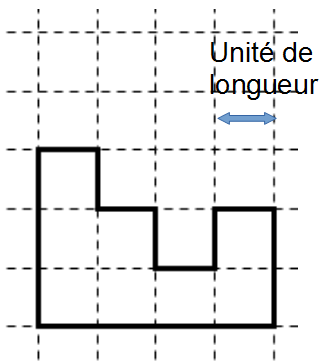
\includegraphics[scale=0.55]{./img/aire}}			
		\end{column}
		\begin{column}{0.465\textwidth}
			Le périmètre de cette figure est 16 unités de longueur.			
		\end{column}
	\end{columns}
		
\end{block}	


\end{frame}

\subsection{Unité de longueur}
\begin{frame}
	\frametitle{}  
	\framesubtitle{}	
	
	\begin{exampleblock}{Définition}
		La mesure d'une \bu{longueur} dépend de l'unité choisie.
		L'unité légale de longueur est le \bu{metre} (m).		
	\end{exampleblock}
	
	\begin{alertblock}{Autres unités de longueur}
		\tiny{\begin{tabular}{|c|c|c|c|c|c|c|}
	\hline
		\rowcolor{gray} \multicolumn{3}{|c|}{\textbf{\underline{Multiples} de l'unité}} & \textbf{Unité} & \multicolumn{3}{c|}{\textbf{\underline{Sous-multiples} de l'unité}} \\
	\hline
		\textbf{Kilo}mètre & \textbf{hecto}mètre & \textbf{déca}mètre & \bu{mètre} & \textbf{déci}mètre & \textbf{centi}mètre & \textbf{milli}mètre \\
	\hline
		1 km $=$ 1 000 m & 1hm $=$ 100 m & 1 dam $=$ 10 m & 1m & 1 dm $=$ 0,1 m & 1 cm $=$ 0,01 m & 1 mm $=$ 0,001 m \\
	\hline
	
\end{tabular}}
	\end{alertblock}
		
\end{frame}

\begin{frame}
	\frametitle{}  
	\framesubtitle{}	
	
	\begin{alertblock}{Autres unités de longueur}
		\tiny{\begin{tabular}{|c|c|c|c|c|c|c|}
	\hline
		\rowcolor{gray} \multicolumn{3}{|c|}{\textbf{\underline{Multiples} de l'unité}} & \textbf{Unité} & \multicolumn{3}{c|}{\textbf{\underline{Sous-multiples} de l'unité}} \\
	\hline
		\textbf{Kilo}mètre & \textbf{hecto}mètre & \textbf{déca}mètre & \bu{mètre} & \textbf{déci}mètre & \textbf{centi}mètre & \textbf{milli}mètre \\
	\hline
		1 km $=$ 1 000 m & 1hm $=$ 100 m & 1 dam $=$ 10 m & 1m & 1 dm $=$ 0,1 m & 1 cm $=$ 0,01 m & 1 mm $=$ 0,001 m \\
	\hline
	
\end{tabular}}
	\end{alertblock}
	
	\begin{columns}[onlytextwidth]
		\begin{column}{0.64\textwidth}
			\begin{block}{Exemple}
				On veut calculer le périmètre de la figure ci-contre : 
				
				\begin{small}
					\begin{itemize}
						\item 32 mm $=$ 3,2 cm et 0,31~dm~$=$~3,1~cm
						\item[P=]  AB + BC + CD + DE + EA
						\item[P=] 2 + 3,2 + 2,2 + 3 + 3,1 
						\item[P=] 13,5
						\item[$\rightarrow$] Le périmètre du polygone ABCDE est 13,5 cm.
					\end{itemize}	
				\end{small}
				
				 
				
				
			\end{block}
		\end{column}
		\begin{column}{0.35\textwidth}
			\center{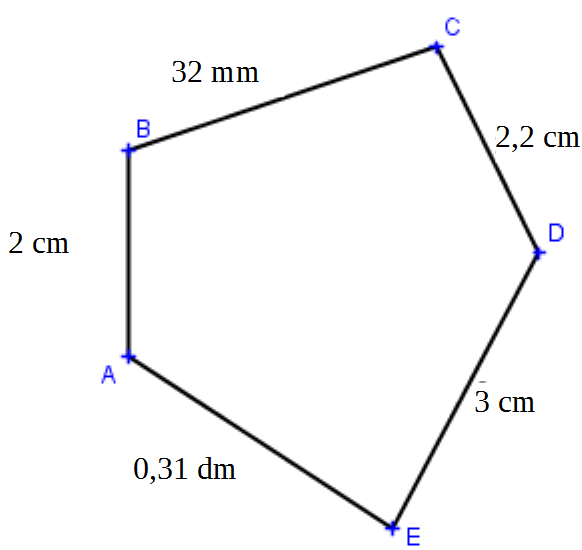
\includegraphics[scale=0.32]{./img/figure}}			
		\end{column}
	\end{columns}
	
\end{frame}

\begin{frame}
	\frametitle{Convertir les unités de longueur}  
	\framesubtitle{À l'aide du tableau de conversion}	
	
	On utilise le tableau ci-dessous :
		\begin{small}
		\begin{center}
			\begin{tabular}{|c|c|c|c|c|c|c|}	
				\hline
					\rowcolor{gray} ~~\textbf{km}~~    &    ~~\textbf{hm}~~ &    ~~\textbf{dam}~~ & ~~\textbf{m}~~ & ~~\textbf{dm}~~ & 	~~\textbf{cm}~~ & ~~\textbf{mm}~~ \\
				\hline
					& & & & & & \\
				\hline	
			\end{tabular}	
		\end{center}
		\end{small}

	
	\begin{block}{Exemple}
		On veut convertir 7,548 hm en m.
		\begin{itemize}
			\item[$\rightarrow$] On met un chiffre par case dans le tableau, en commençant par les unités du nombre de départ. Puis on place la virgule à la nouvelle unité choisie (en ajoutant des zéro si nécessaire)
		\end{itemize}
		
		\begin{small}		
		\begin{center}
			\begin{tabular}{|c|c|c|c|c|c|c|}	
				\hline
				\rowcolor{gray} ~~\textbf{km}~~    &    ~~\textbf{hm}~~ &    ~~\textbf{dam}~~ & ~~\textbf{m}~~ & ~~\textbf{dm}~~ & 	~~\textbf{cm}~~ & ~~\textbf{mm}~~ \\
				\hline
					& 7 & 5 & 4, & 8 & & \\
				\hline	
			\end{tabular}	
		\end{center}
		\end{small}
		
		CONCLUSION : 7,548 hm = 754,8 m.
	\end{block}
	
	
\end{frame}

\begin{frame}
	\frametitle{Convertir les unités de longueur}  
	\framesubtitle{En multipliant ou en divisant directement par 10; 100; 1000 ...}	
	
	\begin{alertblock}{Méthode}
		ON peut convertir directement les unités de longueur à l'aide de multiplications et de divisions par 10; 100; 1000 ...
	\end{alertblock}
	
	\begin{block}{Exemple}
		\begin{itemize}
			\item On veut convertir 32,45 m en cm.
			\item On sait que 1 m $=$ 100 cm.
			\item[$\rightarrow$] 32,45 $\times$ \textbf{100} $=$ 3 245.
		\end{itemize}
		
		Donc 32,45 m $=$ 3 245 cm.		
	\end{block}
	
\end{frame}

\end{document}


\begin{frame}
	\frametitle{}  
	\framesubtitle{}	
	
\end{frame}